%\documentclass[9pt,handout]{beamer}
\documentclass[11pt]{beamer}

%\usepackage[style=alphabetic]{biblatex}

%\usepackage{pgfpages}
%\setbeameroption{show notes on second screen=left}

% Copyright 2004 by Till Tantau <tantau@users.sourceforge.net>.
%
% In principle, this file can be redistributed and/or modified under
% the terms of the GNU Public License, version 2.
%
% However, this file is supposed to be a template to be modified
% for your own needs. For this reason, if you use this file as a
% template and not specifically distribute it as part of a another
% package/program, I grant the extra permission to freely copy and
% modify this file as you see fit and even to delete this copyright
% notice.
%
% Modified by Tobias G. Pfeiffer <tobias.pfeiffer@math.fu-berlin.de>
% to show usage of some features specific to the FU Berlin template.

% altered by someone at TU. fiddled with and fixed some things by 
% Nicolas Werner (some UTF-8 fix, biblatex-biber intro before toc,
% other stuff I can't remember)

% remove this line and the "ucs" option to the documentclass when your editor is not utf8-capable
\usepackage[utf8]{inputenc}
\usepackage[T1]{fontenc}   % to make utf-8 input possible
\usepackage[english]{babel}     % hyphenation etc., alternatively use 'german' as parameter
\usepackage{verbatim}           % comments and stuff
\usepackage[right]{eurosym}
\usepackage{booktabs}
\usepackage{tikz}
\newcommand{\todo}[1]{\raisebox{0pt}{\parbox{0pt}{\begin{large}\colorbox{red}{todo: #1}\end{large} \hspace*{0.05cm}}}}

\usepackage{blindtext}
\usepackage[fixlanguage]{babelbib}
\selectbiblanguage{english}


% ``English''  <>  "`Deutsch"'
\newcommand{\germanQuote}[1]{\glqq#1\grqq}
\newcommand{\englishQuote}[1]{``#1''}
% in Überschriften kann es sein,
% dass man danach $\;$ 
% setzen muss, damit
% die Abstände stimmen.....
% in Sections ist das aber illegal
% deswegen:
% \texorpdfstring{\germanQuote{Text} $\;$blah}{\germanQuote{Text} blah}

%\addbibresource{references.bib}
\bibliographystyle{alpha}
%\bibliography{references}

% Template for talks using the Corporate Design of the Freie Universitaet
%   Berlin, created following the guidelines on www.tu-berlin.de/cd by
%   Tobias G. Pfeiffer, <tobias.pfeiffer@math.tu-berlin.de>
% This file can be redistributed and/or modified in any way you like.
%   If you feel you have done significant improvements to this template,
%   please consider providing your modified version to
%   https://www.mi.tu-berlin.de/w/Mi/BeamerTemplateCorporateDesign

% altered by someone at TU. fiddled with and fixed some things by 
% Nicolas Werner (correct colours, no figure numbering, 
% some more stuff I can't remember)

\usepackage{amsmath,dsfont,listings}
\usetheme{Frankfurt}

\setbeamertemplate{sections/subsections in toc}[default]
\setbeamertemplate{items}[default]
\setbeamertemplate{itemize items}[default]
\setbeamertemplate{enumerate items}[default]


\hypersetup{colorlinks,citecolor={blue},linkcolor={},urlcolor={red}}

%%% TU logo
% small version for upper right corner of normal pages
\pgfdeclareimage[height=0.9cm]{university-logo}{TU_Logo_lang_RGB_rot}
\logo{\pgfuseimage{university-logo}}
% large version for upper right corner of title page
\pgfdeclareimage[height=1.085cm]{big-university-logo}{TU_Logo_lang_RGB_rot}
\newcommand{\titleimage}[1]{\pgfdeclareimage[height=2.92cm]{title-image}{#1}}
\titlegraphic{\pgfuseimage{title-image}}
%%% end TU logo




% NOTE: 1cm = 0.393 in = 28.346 pt;    1 pt = 1/72 in = 0.0352 cm
\setbeamersize{text margin right=3.5mm, text margin left=7.5mm}  % text margin

% colors to be used
\definecolor{text-grey}{rgb}{0.45, 0.45, 0.45} % grey text on white background
\definecolor{bg-grey}{rgb}{0.66, 0.65, 0.60} % grey background (for white text)
\definecolor{tu-blue}{RGB}{0, .2, .4} % blue text
\definecolor{tu-green}{RGB}{.6, .8, 0} % green text
%\definecolor{tu-red}{RGB}{204, 0, 0} % red text (used by \alert)
\definecolor{tu-red}{rgb}{.772, .055, .122}%{0.6,0,0} %% based on DARKRED TU-LOGO -- GIMP says TU DARKRED is RGB{153,0,0}

% switch off the sidebars
% TODO: loading \useoutertheme{sidebar} (which is maybe wanted) also inserts
%   a sidebar on title page (unwanted), also indents the page title (unwanted?),
%   and duplicates the navigation symbols (unwanted)
\setbeamersize{sidebar width left=0cm, sidebar width right=0mm}
\setbeamertemplate{sidebar right}{}
\setbeamertemplate{sidebar left}{}
%    XOR
% \useoutertheme{sidebar}

% frame title
% is truncated before logo and splits on two lines
% if neccessary (or manually using \\)
\setbeamertemplate{frametitle}{%
    \vskip-30pt \color{text-grey}\large%
    \begin{minipage}[b][23pt]{80.5mm}%
    \flushleft\insertframetitle%
    \end{minipage}%
}

%%% title page
% TODO: get rid of the navigation symbols on the title page.
%   actually, \frame[plain] *should* remove them...
\setbeamertemplate{title page}{
	
	% upper right: FU logo
	\hfill\pgfuseimage{big-university-logo} \\
	
	% title image of the presentation
	\begin{minipage}{11.6cm}
		\hspace{-1mm}\vspace{0.5cm}\inserttitlegraphic
	\end{minipage}

	% set the title and the author
	\parbox[top][1.35cm][c]{11cm}{\inserttitle}
	\vskip10pt
	\parbox[top][1.35cm][c]{11cm}{\color{text-grey} {\tiny \insertauthor\\ \insertinstitute\\ \insertdate}}
}
%%% end title page

%%% colors
\usecolortheme{lily}
\setbeamercolor*{normal text}{fg=black,bg=white}
\setbeamercolor*{alerted text}{fg=tu-red}
\setbeamercolor*{example text}{fg=tu-green}
\setbeamercolor*{structure}{fg=tu-blue}

\setbeamercolor*{block title}{fg=white,bg=black!50}
\setbeamercolor*{block title alerted}{fg=white,bg=black!50}
\setbeamercolor*{block title example}{fg=white,bg=black!50}

\setbeamercolor*{block body}{bg=black!10}
\setbeamercolor*{block body alerted}{bg=black!10}
\setbeamercolor*{block body example}{bg=black!10}

\setbeamercolor{bibliography entry author}{fg=tu-blue}
% TODO: this doesn't work at all:
\setbeamercolor{bibliography entry journal}{fg=text-grey}

\setbeamercolor{item}{fg=tu-blue}
%\setbeamercolor{navigation symbols}{fg=text-grey,bg=bg-grey}
\setbeamercolor{navigation symbols}{fg=text-grey,bg=bg-grey}
%%% end colors

%%% headline
\setbeamertemplate{headline}{
\vskip4pt\hfill\insertlogo\hspace{3.5mm} % logo on the right
\vskip6pt\color{tu-red}\rule{\textwidth}{0.4pt} % horizontal line was BLUE!
}

%%% footline
\setbeamercolor{upper separation line head}{bg=red}
\setbeamercolor{section in head/foot}{fg=black, bg=white}
\setbeamercolor{frametitle}{fg=red, bg=white}

\newcommand{\footlinetext}{
	\insertshortinstitute, \insertshorttitle, \insertshortdate
}


\makeatletter
%THIS IS OLD
%\setbeamertemplate{footline}{
%\vskip5pt\color{tu-red}\rule{\textwidth}{0.4pt}\\ % horizontal line
%\vskip2pt
%\makebox[123mm]{\hspace{7.5mm}
%\color{black}\footlinetext
%\hfill \raisebox{-1pt}{\phantom{\usebeamertemplate***{navigation symbols}}}
%%\hfill \raisebox{-1pt}{\phantom{\big{lol}}}%\raisebox{-1pt}{\usebeamertemplate***{navigation symbols}}
%\hfill \insertframenumber}
%\vskip4pt
%}
\setbeamertemplate{footline}{
\vskip5pt\color{tu-red}\rule{\textwidth}{0.4pt}\\ % horizontal line
\pgfuseshading{beamer@barshade}%
  \ifbeamer@sb@subsection%
    \vskip-9.75ex%
  \else%
    \vskip-7ex%
  \fi%
  % fügt die Navigationsleiste ein:
  \begin{beamercolorbox}[ignorebg,dp=3.75ex,ht=2.25ex]{subsection in head/foot}
	\insertnavigation{0.5\paperwidth} % <======= Added 0.5 here
  \end{beamercolorbox}%
  % kein Plan was das macht :D
  \ifbeamer@sb@subsection%
    \begin{beamercolorbox}[ignorebg,ht=2.125ex,dp=1.125ex,%
      leftskip=.3cm,rightskip=.3cm plus1fil]{subsection in head/foot}
      \usebeamerfont{subsection in head/foot}\insertsubsectionhead
    \end{beamercolorbox}%
  \fi%
  %
  % GROßE Trennlinie:
  %\begin{beamercolorbox}[colsep=1.5pt,ht=.75ex]{upper separation line head}
  %\end{beamercolorbox}
  \vskip-2ex%
  \hskip0.98\textwidth \insertframenumber % hfill
  \vskip4pt % vom unteren Rand 4 pt weg
}

\makeatother
%%% end footline

%%% settings for listings package
\lstset{extendedchars=true, showstringspaces=false, basicstyle=\footnotesize\sffamily, tabsize=2, breaklines=true, breakindent=10pt, frame=l, columns=fullflexible}
\lstset{language=Java} % this sets the syntax highlighting
\lstset{mathescape=true} % this switches on $...$ substitution in code
% enables UTF-8 in source code:
\lstset{literate={ä}{{\"a}}1 {ö}{{\"o}}1 {ü}{{\"u}}1 {Ä}{{\"A}}1 {Ö}{{\"O}}1 {Ü}{{\"U}}1 {ß}{\ss}1}


%%% end listings
  % THIS is the line that includes the TU template!
% Quelle: http://tex.stackexchange.com/questions/56417/list-of-figures-beamer
\usepackage{ifthen}
\usepackage{xstring}

\makeatletter

%\defbeamertemplate*{caption label separator}{colon}{:}

\def\dotfill{%
  \leavevmode
  \cleaders \hb@xt@ .44em{\hss.\hss}\hfill
  \kern\z@}

\newcommand{\myVL}[2]{\tmpVL{#1}{#2}}

\newcommand{\tmpVL}[2]{Page #1, last accessed: #2}

\newcommand{\myhref}[2]{\tmphref{#1}{#2}}

\newcommand{\tmphref}[2]{\href{#1}{Source}, last accessed: #2}

\AtEndDocument{%
  % sorgt dafür, dass die Dateien 
  % *.lof -> list of figures
  % *.lot -> list of tables
  % geeleert werden oder ggf. neu erzeugt werden (erzwungen)
  \clearpage
  \beamer@tempcount=\c@page\advance\beamer@tempcount by -1%
  \if@filesw
  \newwrite\tf@lof
  \immediate\openout\tf@lof\jobname.lof\relax
  \newwrite\tf@lot
  \immediate\openout\tf@lot\jobname.lot\relax
  \fi
}

% beamer caption ändern....
\long\def\beamer@makecaption#1#2#3#4{%
  % [ von caption selbst]
  % #1 == Typ == Bild / Tabelle....
  % #2 == optionale Beschreibung
  % #3 == caption Beschreibung
  % bsp: \caption[optionale Beschreibung]{caption Beschreibung}

  % calls: \beamer@makecaption{#1}{\ignorespaces #3}{yes/no}{\ignorespaces #2}  

  % ----------------------------------------------

  % #1 == Typ == Tabelle / Bild.....
  % #2 == Captionbeschreibung
  % #3 == yes/no if you want complete Text under picture
  % #4 == optionale Beschreibung vom Bild
  \hypertarget{\insertframenumber}{}{}
  % \def\insertcaptionname{\csname#1name\endcsname}%
  % liefert Figure, weil babel auf englisch....
  \def\insertcaptionname{Fig.}%
  \def\insertcaptionnumber{\csname the#1\endcsname}%
  \edef\insertframenumber{\theframenumber}%
%  \ifthenelse{\equal{#3}{\empty}}{%  
    \def\insertlistcaption{#2}%
%  }{%
%    \def\insertlistcaption{#3}%
%  }
  	\def\insertsource{#4}%
    %
    \def\insertcaption{#2}%
    \ifthenelse{\equal{#1}{figure}}{%  
      \addtocontents{lof}{\relax\protect\listoffigureformat{\insertcaptionnumber}{\insertlistcaption}{\protect\hyperlink{\insertframenumber}{\insertframenumber}}{\insertsource}}{}{}%
      }{}
    \ifthenelse{\equal{#1}{table}}{%  
      \addtocontents{lot}{\protect\listoftableformat{\insertcaptionnumber}{\insertlistcaption}{\insertframenumber}}{}{}%
      }{}
  \ifthenelse{\equal{#3}{no}}
  { 
  	% Text beim Bild
    %\addtocontents{lof}{#4,jaaaaaaaaaaaaaaaaaaaaaaa}%
  	\nobreak\vskip\abovecaptionskip\nobreak
  	\sbox\@tempboxa{
  		%\usebeamertemplate**{caption}
  		%\raggedright
    	{%	
      		\usebeamercolor[fg]{caption name}%
      		\usebeamerfont*{caption name}%
      		\insertcaptionname~\insertcaptionnumber
    	}
    	\par
  	}%
  	\ifdim \wd\@tempboxa >\hsize
    	%\usebeamertemplate**{caption}\par
    	%\raggedright
    	{%
      		\usebeamercolor[fg]{caption name}%
      		\usebeamerfont*{caption name}%
      		\insertcaptionname~\insertcaptionnumber
    	}
    	\par
 	\else
  		\global \@minipagefalse
  		\hb@xt@\hsize{\hfil\box\@tempboxa\hfil}%
  	\fi
  	\nobreak\vskip\belowcaptionskip\nobreak%
  }{ 
	% Text beim Bild
    %\addtocontents{lof}{#4,jaaaaaaaaaaaaaaaaaaaaaaa}%
  	\nobreak\vskip\abovecaptionskip\nobreak
  	\sbox\@tempboxa{
  		%\usebeamertemplate**{caption}
  		%\raggedright
    	{%	
% % nw: figure numbering in slides
%      		\usebeamercolor[fg]{caption name}%
%      		\usebeamerfont*{caption name}%
%      		\insertcaptionname~\insertcaptionnumber
%      		\usebeamertemplate{caption label separator}%
    	}
    	\insertcaption\par
  	}%
  	\ifdim \wd\@tempboxa >\hsize
    	%\usebeamertemplate**{caption}\par
    	%\raggedright
    	{%
      		\usebeamercolor[fg]{caption name}%
      		\usebeamerfont*{caption name}%
      		\insertcaptionname~\insertcaptionnumber
      		\usebeamertemplate{caption label separator}%
    	}
    	\insertcaption\par
 	\else
  		\global \@minipagefalse
  		\hb@xt@\hsize{\hfil\box\@tempboxa\hfil}%
  	\fi
  	\nobreak\vskip\belowcaptionskip\nobreak%  }
  }
}

\def\listoffiguresectionformat#1#2{%
  % \listoffiguresectionformat{\insertsectionhead}{\insertframenumber}
  % #1 == Sectiontitel
  % #2 == Seite
  \setlength{\leftskip}{2ex}
  \setlength{\rightskip}{-0.6ex}
  \setlength{\parindent}{-3ex}
  %
  {\usebeamercolor[fg]{bibliography entry author} #1}%
  \dotfill%
  \hspace*{0.6ex}%
  \makebox[3ex][r]{#2}\par%
  %
  \setlength{\leftskip}{3ex}
  \setlength{\rightskip}{0ex}
  \setlength{\parindent}{-3ex}
}

\newcounter{tmpImageCounter}
\setcounter{tmpImageCounter}{0}

\def\listoffigureformat#1#2#3#4{%
	\ifnum\value{tmpImageCounter}=#1
		\typeout{Counter \thetmpImageCounter  ist gleich #1. Das Muss das erste Bild sein...}
		% \listoffigureformat{\insertcaptionnumber}{\insertlistcaption}{\insertframenumber}{\insertsource}
		% #1 == Bildnummer
		% #2 == Captionbeschreibung
		% #3 == Seite, wo das Bild ist
		% #4 == optionale Beschreibung vom Bild 
		% \caption[optionale Beschreibung]{Captionbeschreibung}
		\makebox[2ex][r]{#1}%
		\hspace{1ex}%
		{\usebeamercolor[fg]{bibliography entry author} #2}%
		\ifthenelse{\equal{#4}{\empty}}{}{ -- #4}%
		\dotfill%
		\makebox[3ex][r]{#3}\par%
		\refstepcounter{tmpImageCounter}
	% Bild wurde schonmal gesetzt....nee nicht nochmal...
  	\else
		\PackageWarning{listoffigureformat}{Bild wurde doppelt gesetzt -- wird ignoriert!}
		\typeout{Counter \thetmpImageCounter ist groesser oder kleiner #1.}
	\fi

}

% der eigentliche Befehl, der am Ende die Liste der Figures anzeigt
\def\listoffigures{%
  \setlength{\leftskip}{3ex}
  \setlength{\parindent}{-3ex}
  \@starttoc{lof}%
}

\def\listoftableformat#1#2#3{%
 % \listoftableformat{\insertcaptionnumber}{\insertlistcaption}{\insertframenumber}
 % #1 == Tabellennummer
 % #2 == Captionbeschreibung 
 % #3 == Seite, wo die Tabelle ist
 \makebox[2ex][r]{#1}\hspace{1ex}#2\dotfill\makebox[2ex][r]{#3}\par
}

\def\listoftables{%
  \setlength{\leftskip}{3ex}
  \setlength{\parindent}{-3ex}
  \@starttoc{lot}%
}

% den eigentlichen Caption Befehl umschreiben
\long\def\@caption#1[#2]#3{
  % #1 == Typ == Bild / Tabelle....
  % #2 == optionale Beschreibung
  % #3 == caption Beschreibung
  % bsp: \caption[optionale Beschreibung]{caption Beschreibung}
  \par\nobreak
  \begingroup
    \@parboxrestore
    \if@minipage
      \@setminipage
    \fi
    \beamer@makecaption{#1}{\ignorespaces #3}{yes}{\ignorespaces  #2}\par\nobreak
    \endgroup
}

\def\nocaption{\refstepcounter\@captype\@dblarg{\@nocaption\@captype}}

\long\def\@nocaption#1[#2]#3{
  % #1 == Typ == Bild / Tabelle....
  % #2 == optionale Beschreibung
  % #3 == caption Beschreibung
  % bsp: \caption[optionale Beschreibung]{caption Beschreibung}
  \par\nobreak
  \begingroup
    \@parboxrestore
    \if@minipage
      \@setminipage
    \fi
    \beamer@makecaption{#1}{\ignorespaces #3}{no}{\ignorespaces #2}\par\nobreak
    \endgroup
}



\makeatother


\setbeamertemplate{caption}[numbered]
%\captionsetup{labelformat=simple}
%\setbeamerfont{caption}{size=\TINY}

\usepackage{arev,t1enc,textcomp} % looks nicer than the standard sans-serif font
% if you experience problems, comment out the line above and change
% the documentclass option "9pt" to "10pt"
\usepackage{caption}

\usepackage{xpatch}
\xpatchcmd{\itemize}
  {\def\makelabel}
  {\setlength{\itemsep}{3ex}\def\makelabel}
  {}
  {}


% image to be shown on the title page (without file extension, should be pdf or png)

\titleimage{img/snet_logo} 

\title{Internet of Services Lab - Indoor Navigation}

\subtitle{\small{Indoor Navigation in the TU-Mensa}}

\author[Oldenburg, Hechenberger, Meznarič, Lukau]{{Lennart Oldenburg, Andreas Hechenberger, Jan Meznarič, Eridy Lukau}}

\institute[TU Berlin]{Department of Telecommunication Systems Service-centric Networking 
\\ Technische Universität Berlin}

\date[WS 2015/2016]{WS 2015/2016}

\subject{SNET IoSL Project -- WS 2015/2016}

\renewcommand{\footlinetext}{\insertshortinstitute, \insertshorttitle, \insertshortdate}

\newcounter{currentOutline}

\graphicspath{{./img/}}

\setbeamerfont{caption name}{size=\huge}

\setbeamertemplate{blocks}[rounded][shadow=false] % pdfpc fucks up the shadows, can be true for other viewers

\setbeamertemplate{footline}[text line]{%
    %\parbox{0pt}{\vspace*{-20pt}\hspace*{-23pt}\color{tu-red}\rule{1.2\paperwidth}{0.4pt}}
    \parbox{\linewidth}{%
        \color{text-grey}{%
            \vspace*{-10pt}%
            %WS 2015/2016%
            %\hfill%
            \insertsection%
            \hfill%
            \parbox{0pt}{%
                \vspace*{-3pt}\hspace*{-90pt}%
                
\includegraphics[width=0.1\textwidth]{t-labs_logo}%
                
\includegraphics[width=0.15\textwidth]{snet_logo_long}%
                \hspace{2ex}%
            }\insertpagenumber%
        }%
    }%
}
%\setbeamertemplate{navigation symbols bibliography entry title}{}
\setbeamertemplate{navigation symbols}{}

%fuer umrandeten text

\usepackage[framemethod=TikZ]{mdframed}
\usetikzlibrary{shadows}
\usetikzlibrary{positioning}
\usepackage{environ}
\usepackage{varwidth}
%\usepackage{showframe}

\newlength{\MyMdframedWidthTweak}%
\NewEnviron{bubble}[1][]{%
    \setlength{\MyMdframedWidthTweak}{\dimexpr%
        +\mdflength{innerleftmargin}
        +\mdflength{innerrightmargin}
        +\mdflength{leftmargin}
        +\mdflength{rightmargin}
        }%
    \savebox0{%
        \begin{varwidth}{\dimexpr\linewidth-\MyMdframedWidthTweak\relax}%
            \BODY
        \end{varwidth}%
    }%
    \begin{mdframed}[
        backgroundcolor=lightgray, 
        shadow=true, 
        shadowsize=4pt,
        roundcorner=5pt,
        userdefinedwidth=\dimexpr\wd0+\MyMdframedWidthTweak\relax, 
        #1]
        \usebox0
    \end{mdframed}
}

\usepackage{fancybox}


\begin{document}

\begin{frame}[plain]
    \titlepage
\end{frame}


\stepcounter{currentOutline} % currentOutline = currentOutline + 1
% \setcounter{currentOutline}{value}
% \addtocounter{currentOutline}{value}


% Section: group of navigation bubbles
% Subsection: subgroup of navigation bubbles; black outline instead of grey

\section{Problem scenario \& questions}

\begin{frame}{Use case}

	\vspace{1cm}
	
    \begin{center}

        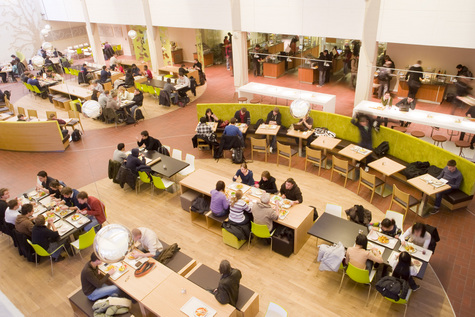
\includegraphics[width=.5\textwidth]{mensa}
        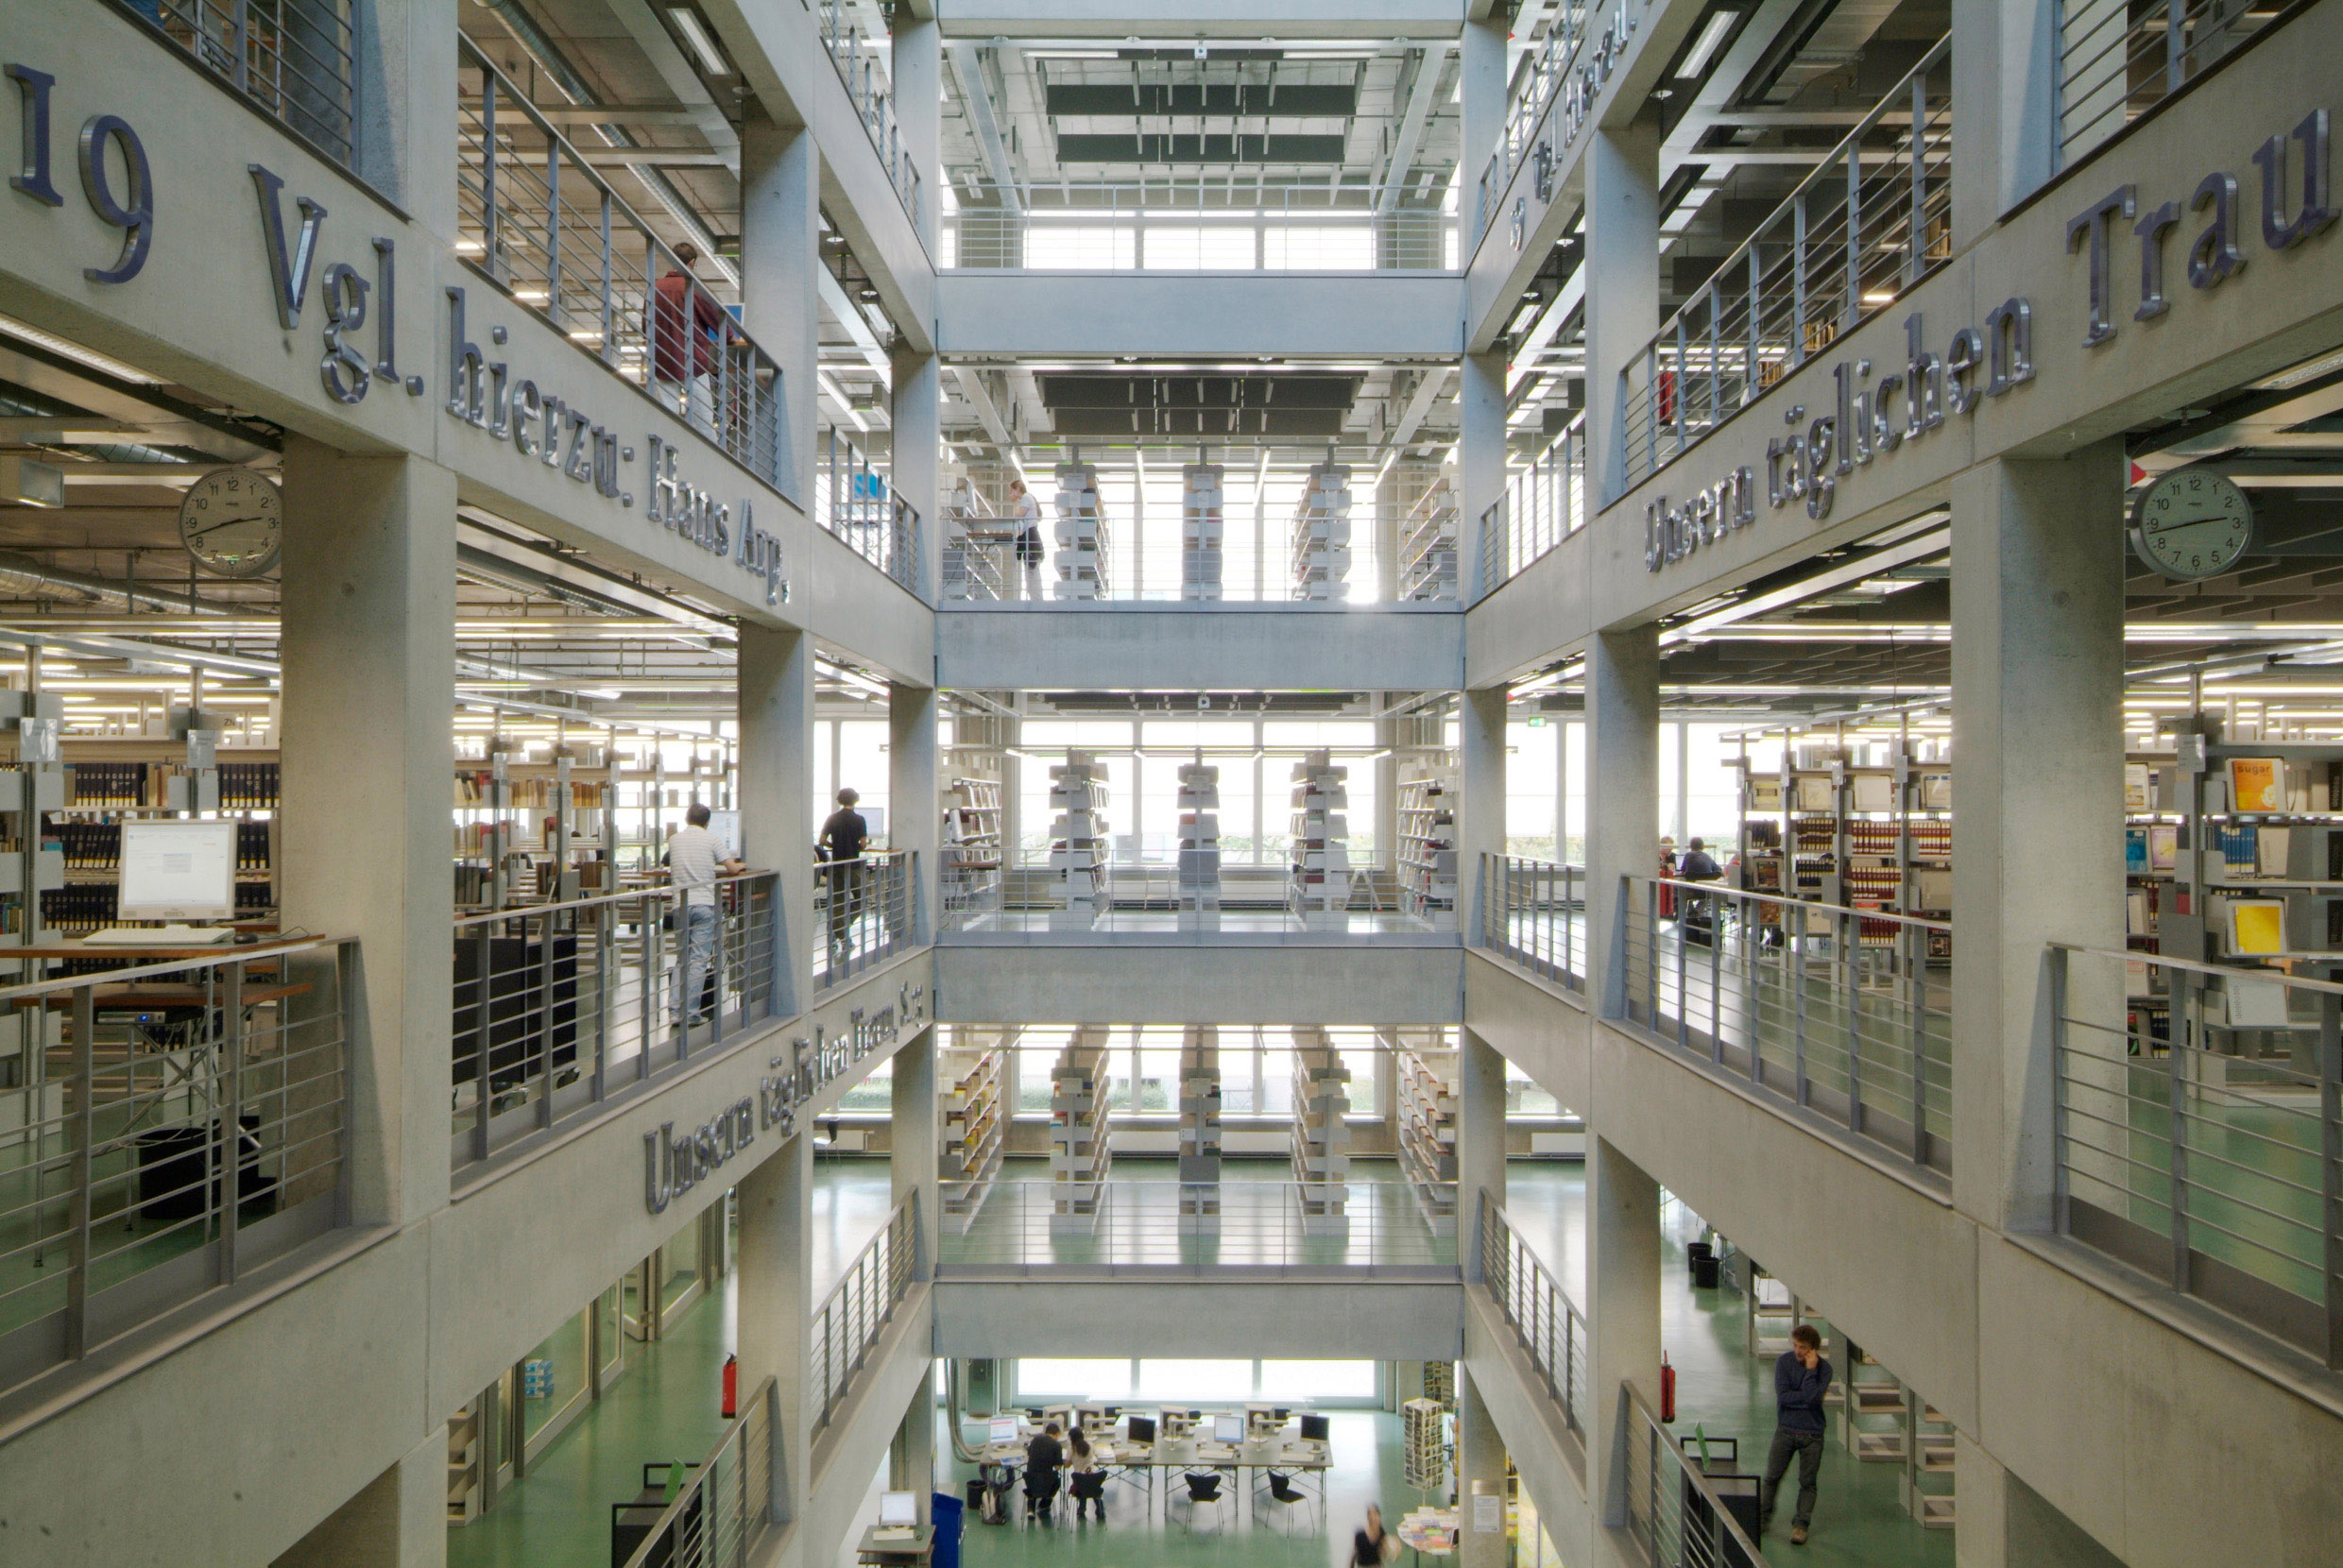
\includegraphics[width=.5\textwidth]{Bibliothek}
    
    \end{center}

	\vspace{1cm}
    
    \tiny{Source left: \url{http://www2.studentenwerk-berlin.de/uploads/pic_untenvonoben_737_full.jpg}}\\
    \tiny{Source right: \url{http://www.berlin-studis.de/images/stories/TU-Universitaetsbibliothek.jpg}}

\end{frame}

\begin{frame}{Use case}

	\begin{center}

        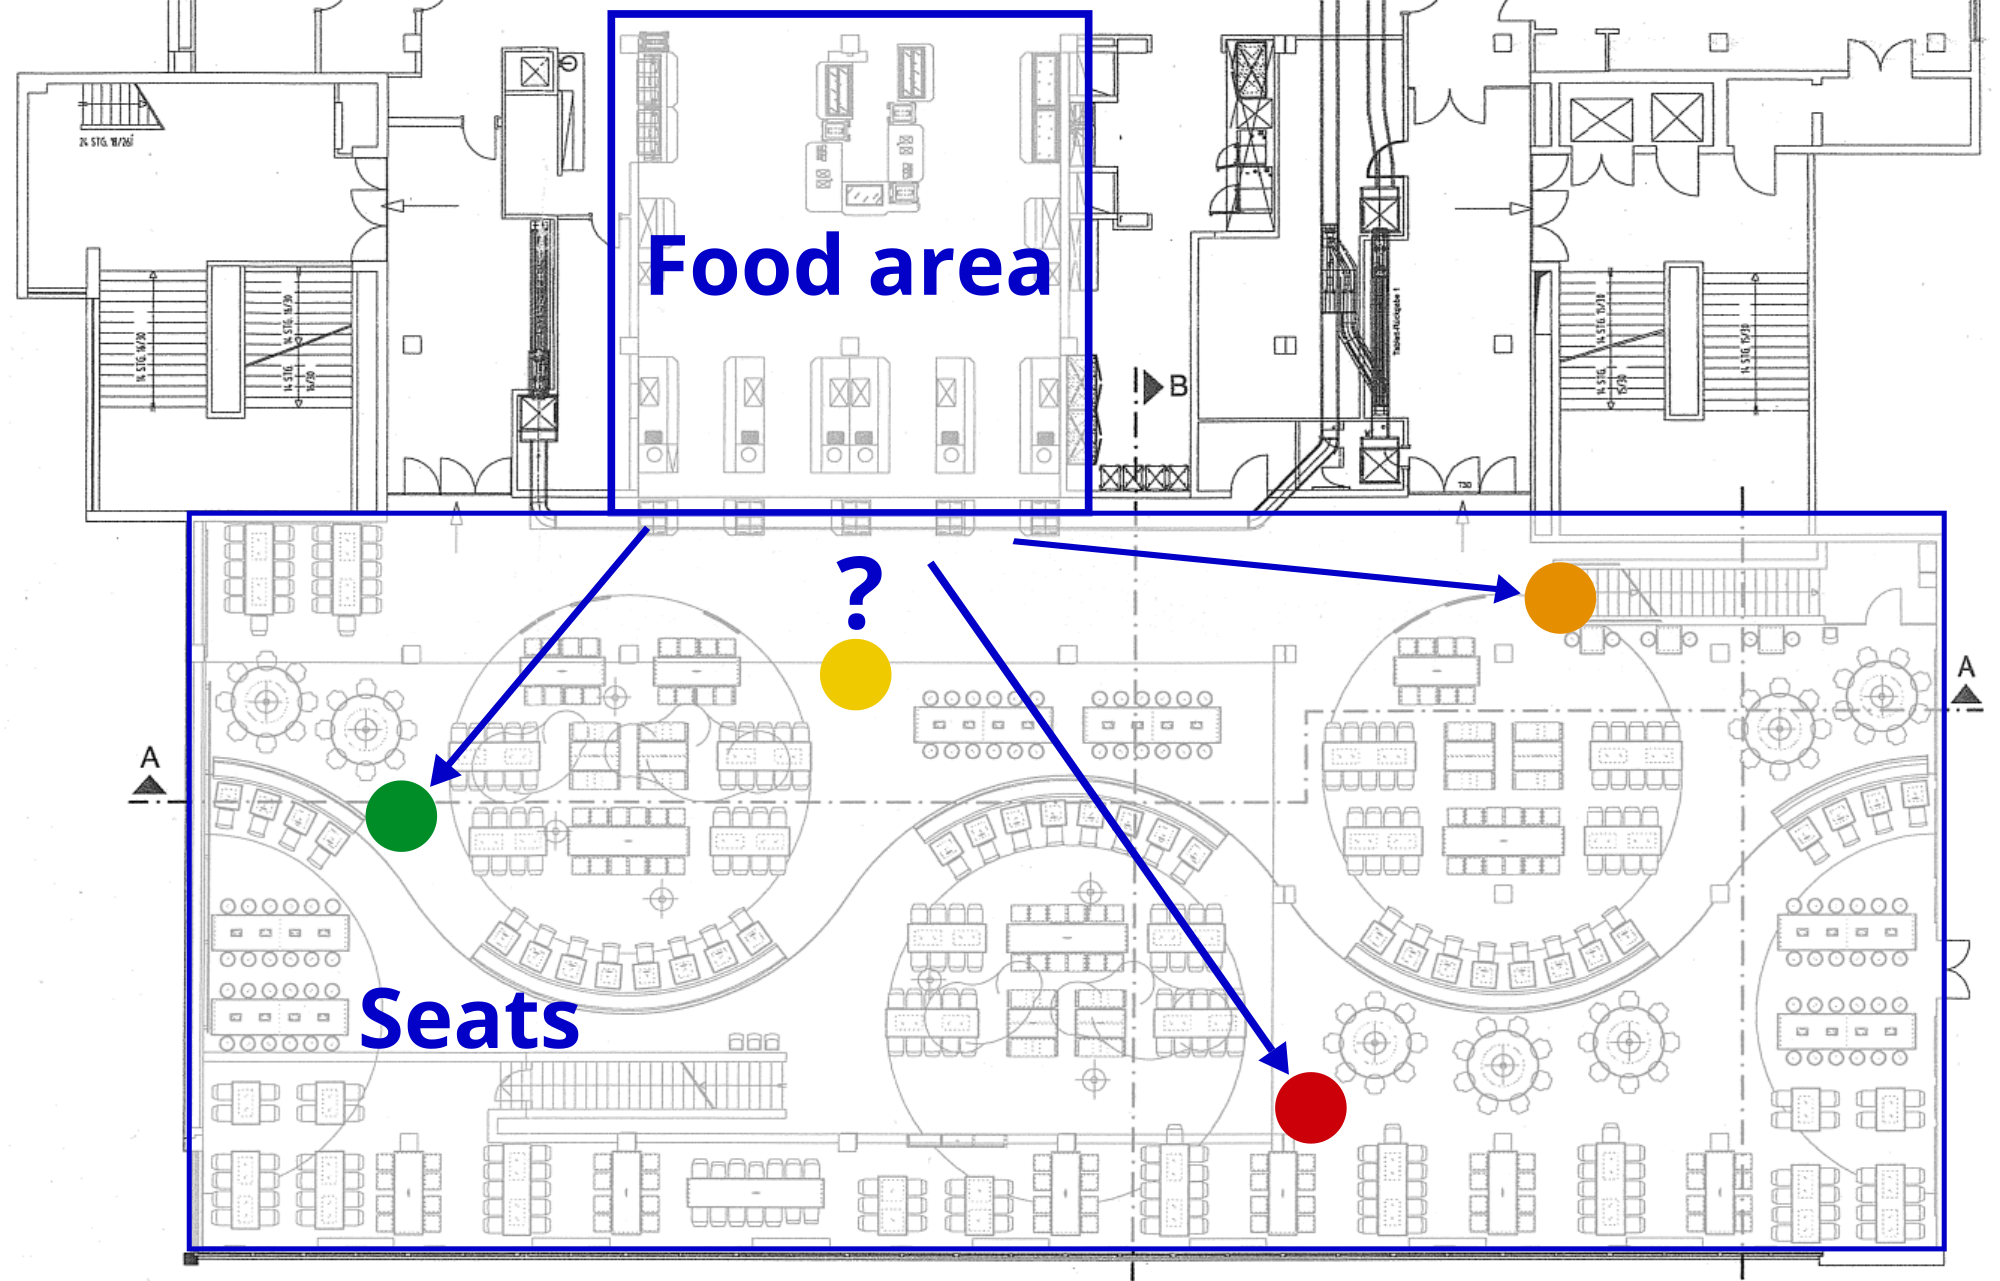
\includegraphics[width=\textwidth]{mensa-floor-plan-people-moving}
    
    \end{center}

\end{frame}

\begin{frame}{App idea}

    \begin{center}

        \vspace*{-14pt}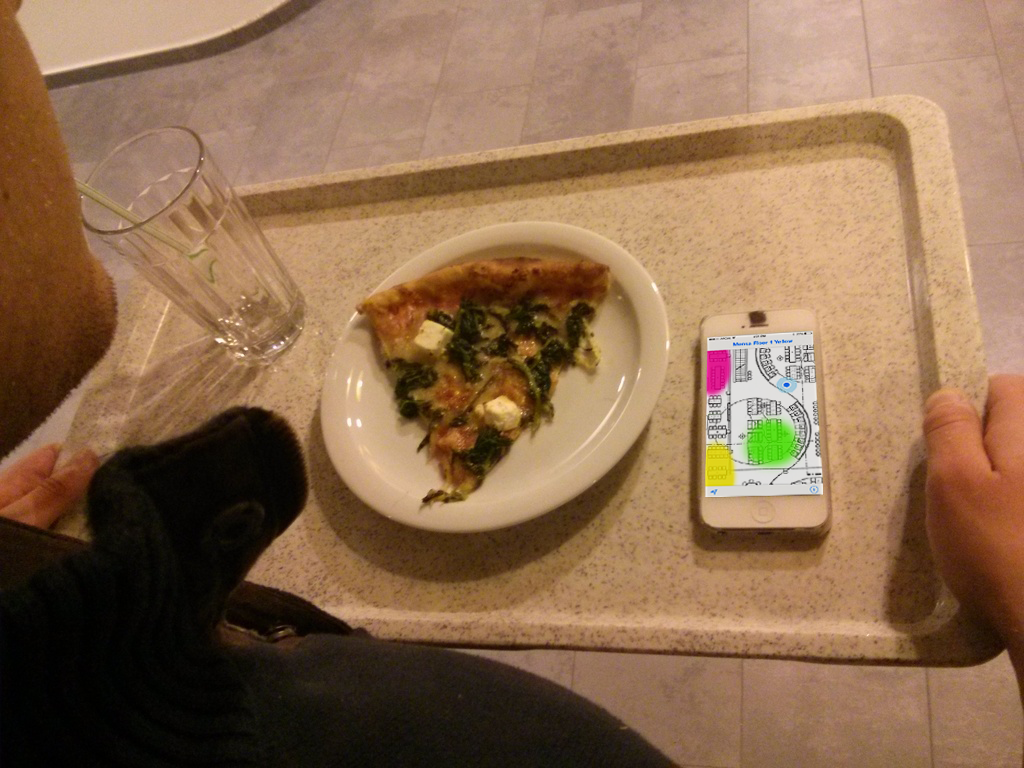
\includegraphics[width=0.8\textwidth]{navitablet}
    
    \end{center}
    
\end{frame}

\begin{frame}{Requirements}

    \begin{itemize}
    
    	\item Fallback when no localization available
    	\item Little interaction
    	\item ...
    
    \end{itemize}

\end{frame}

\section{Technology overview}

\begin{frame}{Localization ideas}

\begin{center}
        \begin{minipage}[b]{0.45\linewidth}
            \begin{minipage}[b]{0.45\linewidth}
                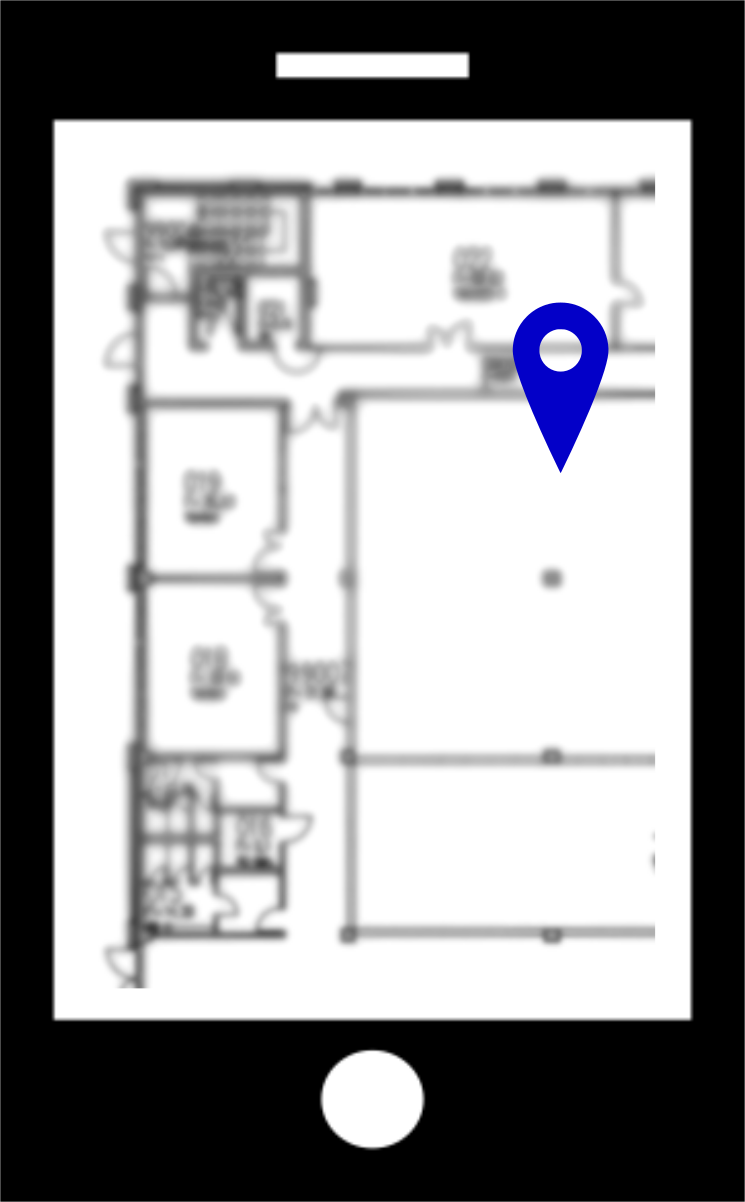
\includegraphics[width=\textwidth]{localisation_manual}
            \end{minipage}%
            \begin{minipage}[b]{0.75\linewidth}
                \begin{itemize}
                    \item manual \\position \\pinning
                \end{itemize}
            \end{minipage}
        \end{minipage}%
            \uncover<2->{
        \begin{minipage}[b]{0.45\linewidth}
            \begin{minipage}[b]{0.45\linewidth}
                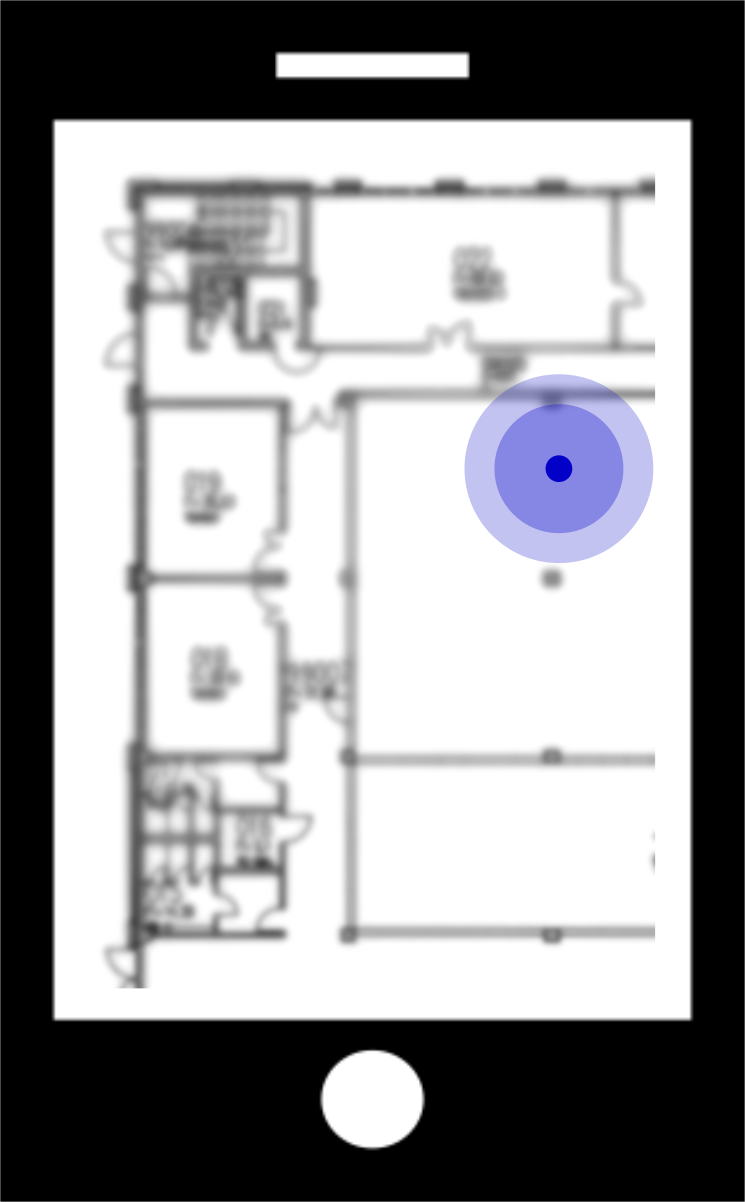
\includegraphics[width=\textwidth]{localisation_automatic}
            \end{minipage}%
            \begin{minipage}[b]{0.75\linewidth}
                \begin{itemize}
                    \item use indoor \\location \\localization
                \end{itemize}
            \end{minipage}
        \end{minipage}
            }
\end{center}
    
\end{frame}

\begin{frame}{Approaches to indoor positioning}

	\begin{itemize}
	
		\item Manual position pinning
		\begin{itemize}
			\setlength{\itemsep}{0.2ex}
			\item Fallback option, if no location available
			\item Pin own location inside mobile application
			\item Alternative for users with high privacy concerns
		\end{itemize}
		
		\item Localization technique
	
	\end{itemize}
	
	\only<2>{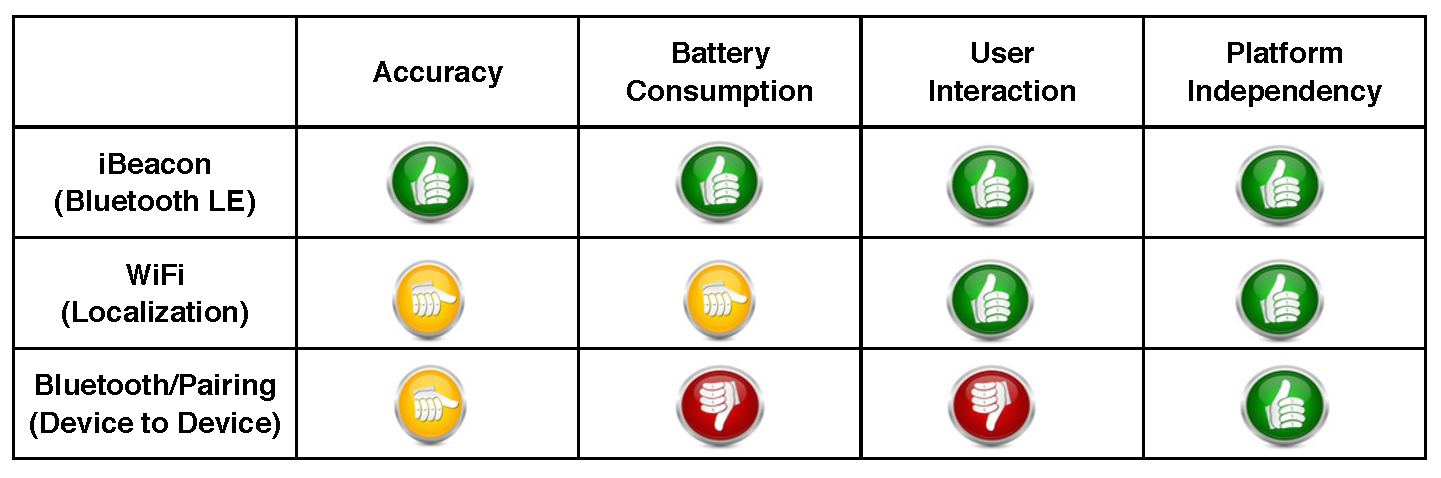
\includegraphics[width=\textwidth]{matrix_zweiteVersion_unhighlighted}}
    \uncover<3>{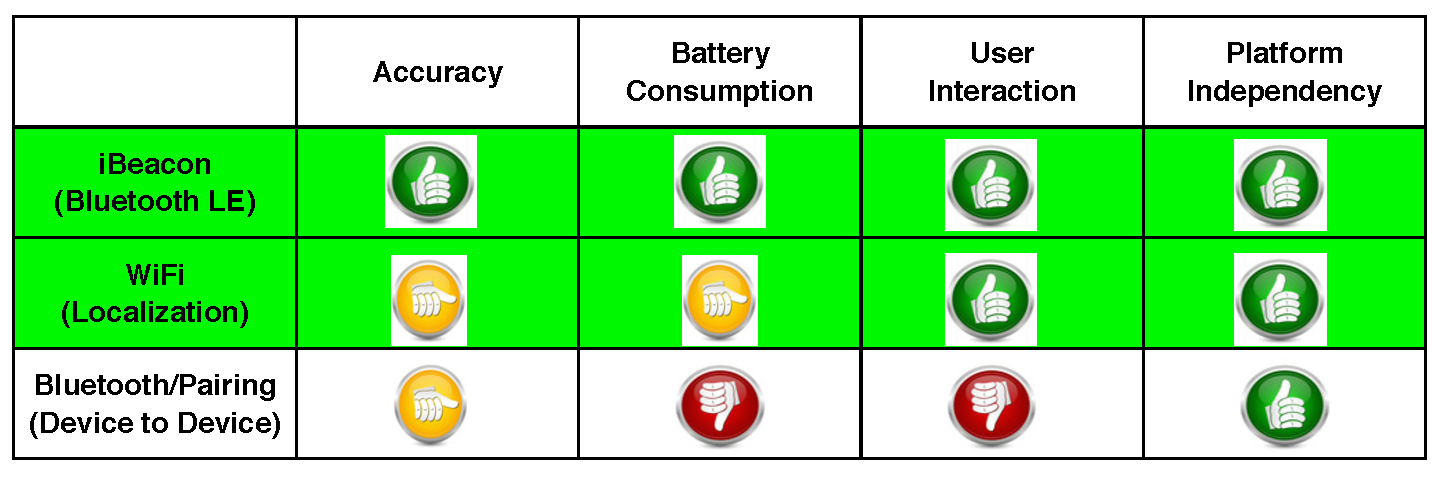
\includegraphics[width=\textwidth]{matrix_zweiteVersion_wifi_beacon_highlighted}}

\end{frame}

\begin{frame}{WiFi positioning via \textbf{CISCO MSE API}}
    
    \uncover<1-> {
	    
	    \begin{itemize}
	    
	        \item For rough positioning
	        \item Uses Cisco Mobility Services Engine
	        \item Provides building name, floor, coordinates
    	    \item Problem: No coordinates in mensa and library
    
	    \end{itemize}
	}
    
    \uncover<2-> {
    
    	\begin{center}
	    
	        
\includegraphics[width=\textwidth]{tubitapi_response}
		   
	    \end{center}
	
	}
    
\end{frame}

\begin{frame}{Bluetooth (Low Energy)}
	
	\begin{columns}[onlytextwidth]

		\begin{column}{.45\textwidth}
		
			\textbf{Estimote} beacons

			\vspace{0.5cm}
			
			\begin{itemize}
				\setlength{\itemsep}{0.75ex}
				\item Precise positioning
				\item iBeacon protocol
			\end{itemize}
			
		\end{column}
		
		\begin{column}{.55\textwidth}
		
			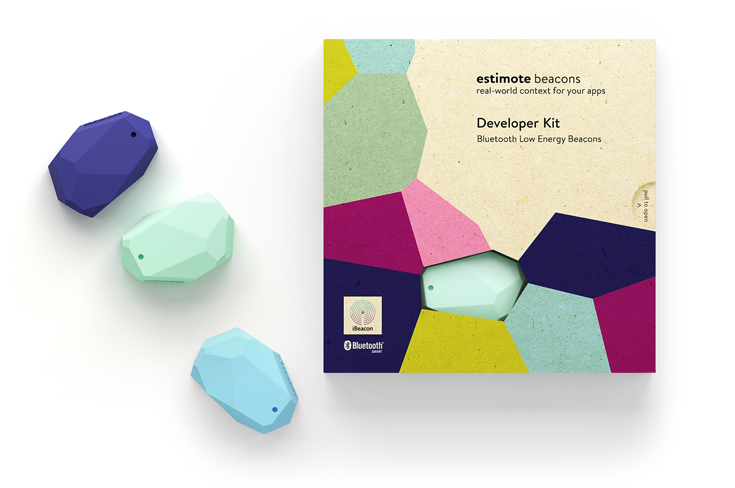
\includegraphics[width=\textwidth]{box_devkit}
			
		\end{column}
	
	\end{columns}

\end{frame}

\begin{frame}{Bluetooth (Low Energy)}
	
	\large Indoor region-based navigation
	\begin{center}
	
		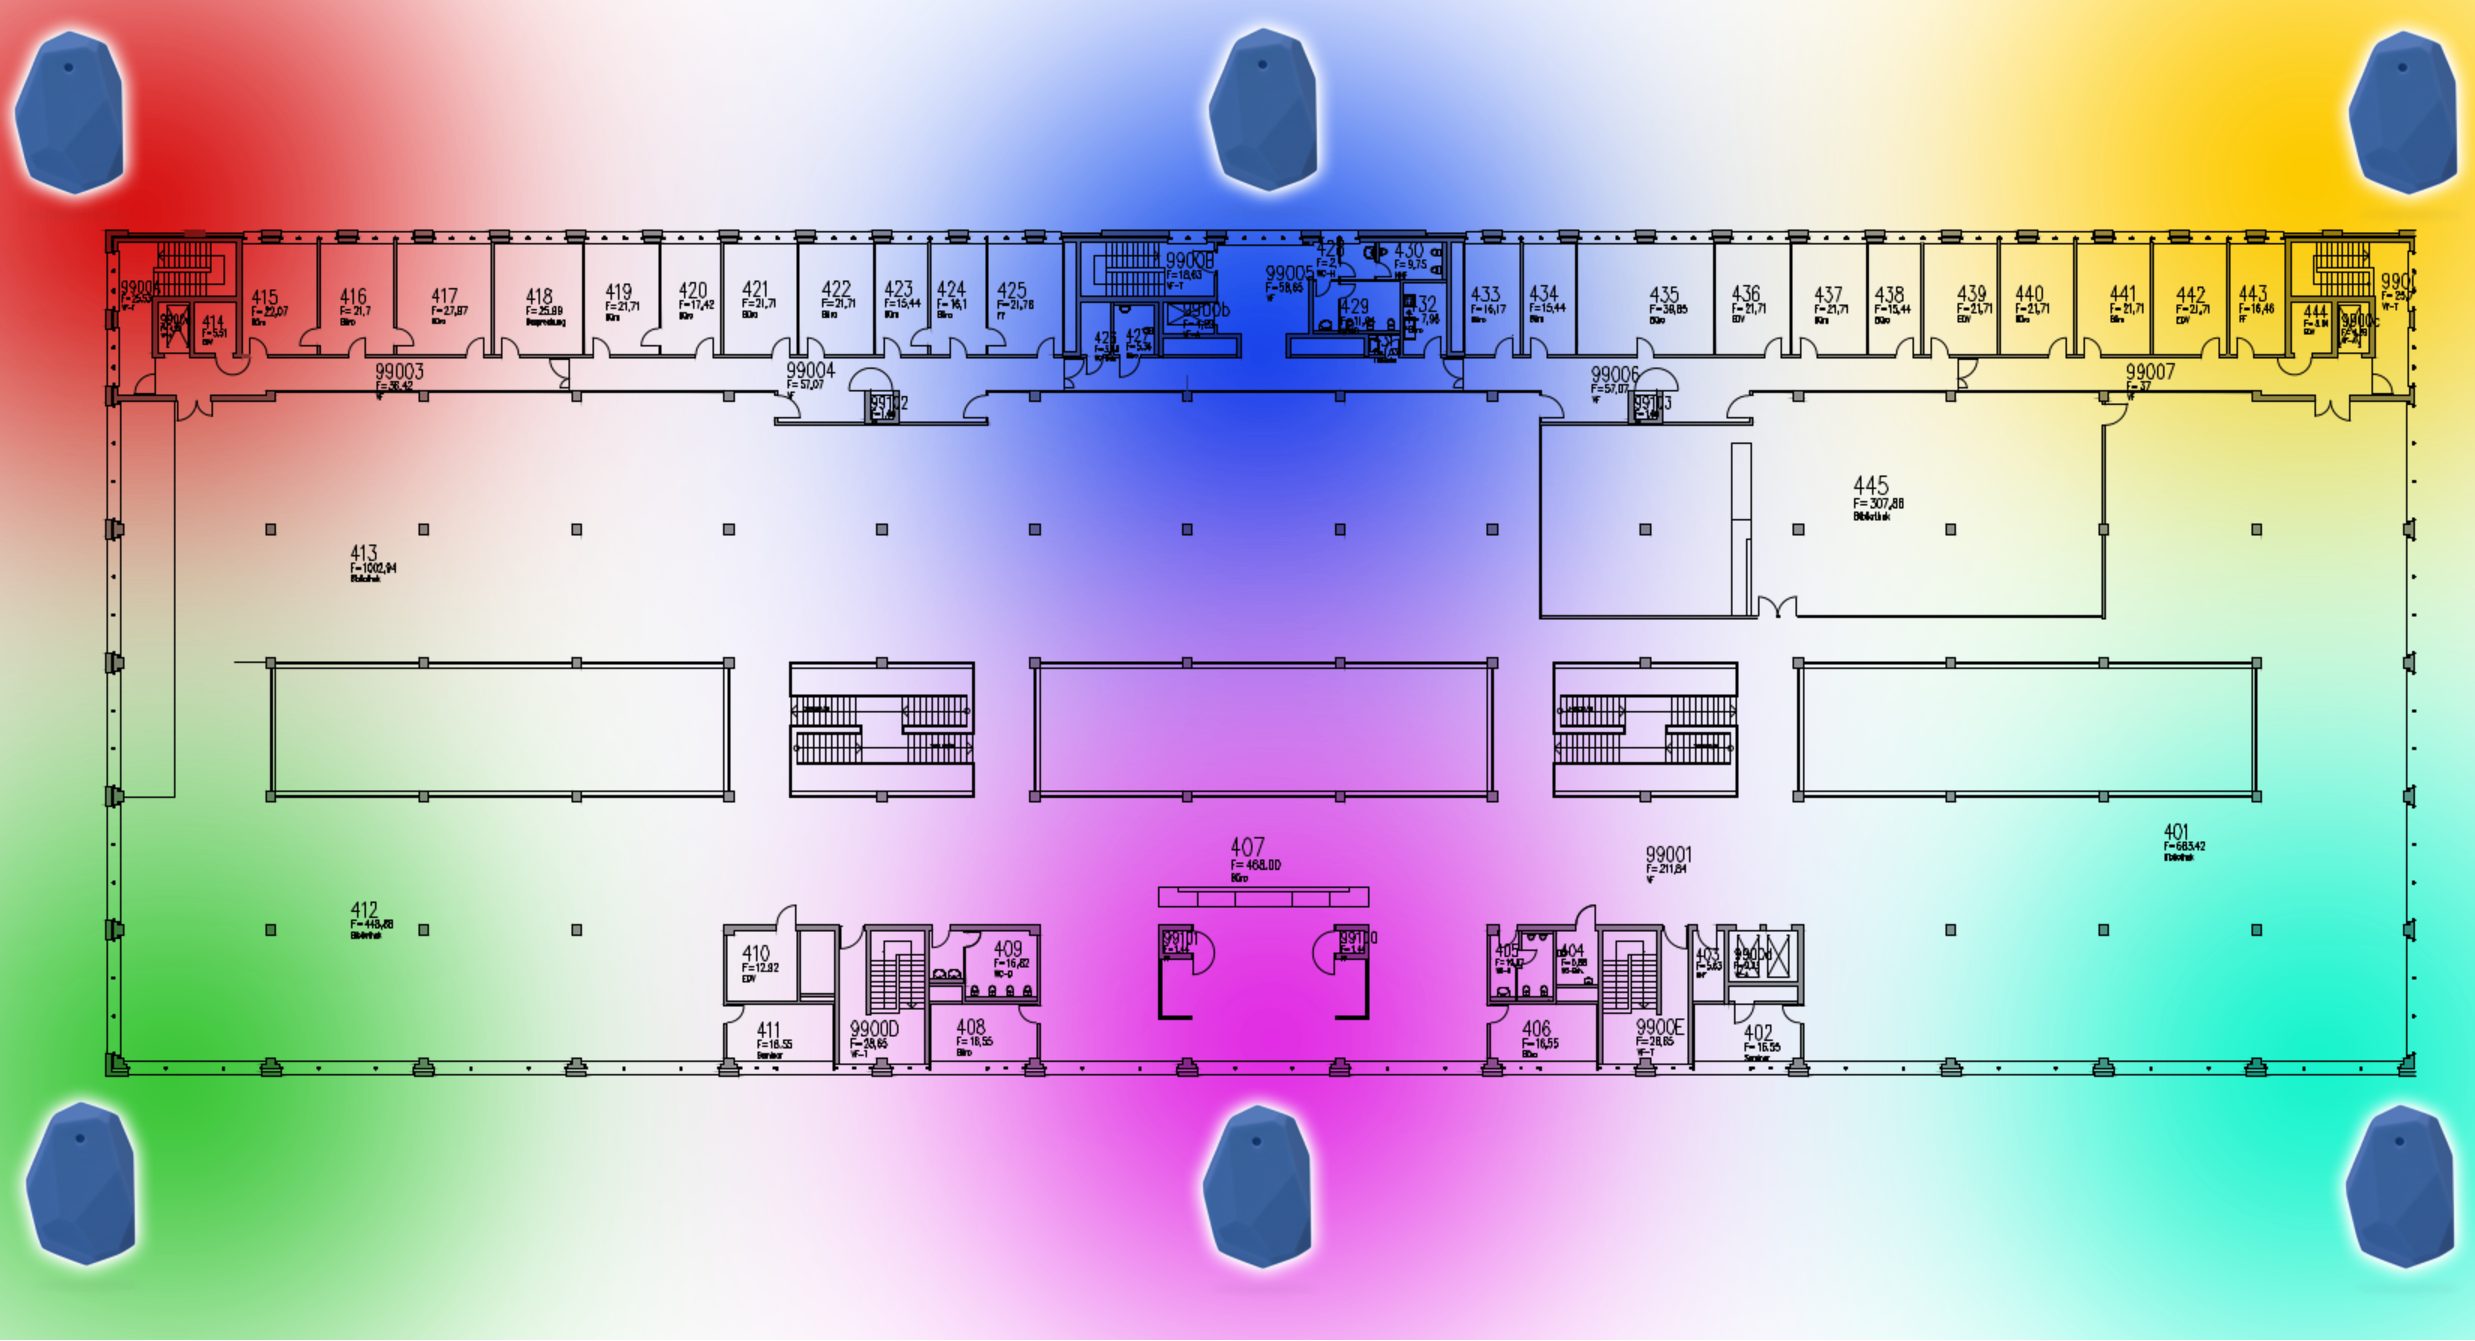
\includegraphics[width=\textwidth]{regions}
	
	\end{center}

\end{frame}

\begin{frame}{User stories}
    
    \textbf{Share location with friends:}

	\begin{center}
	
		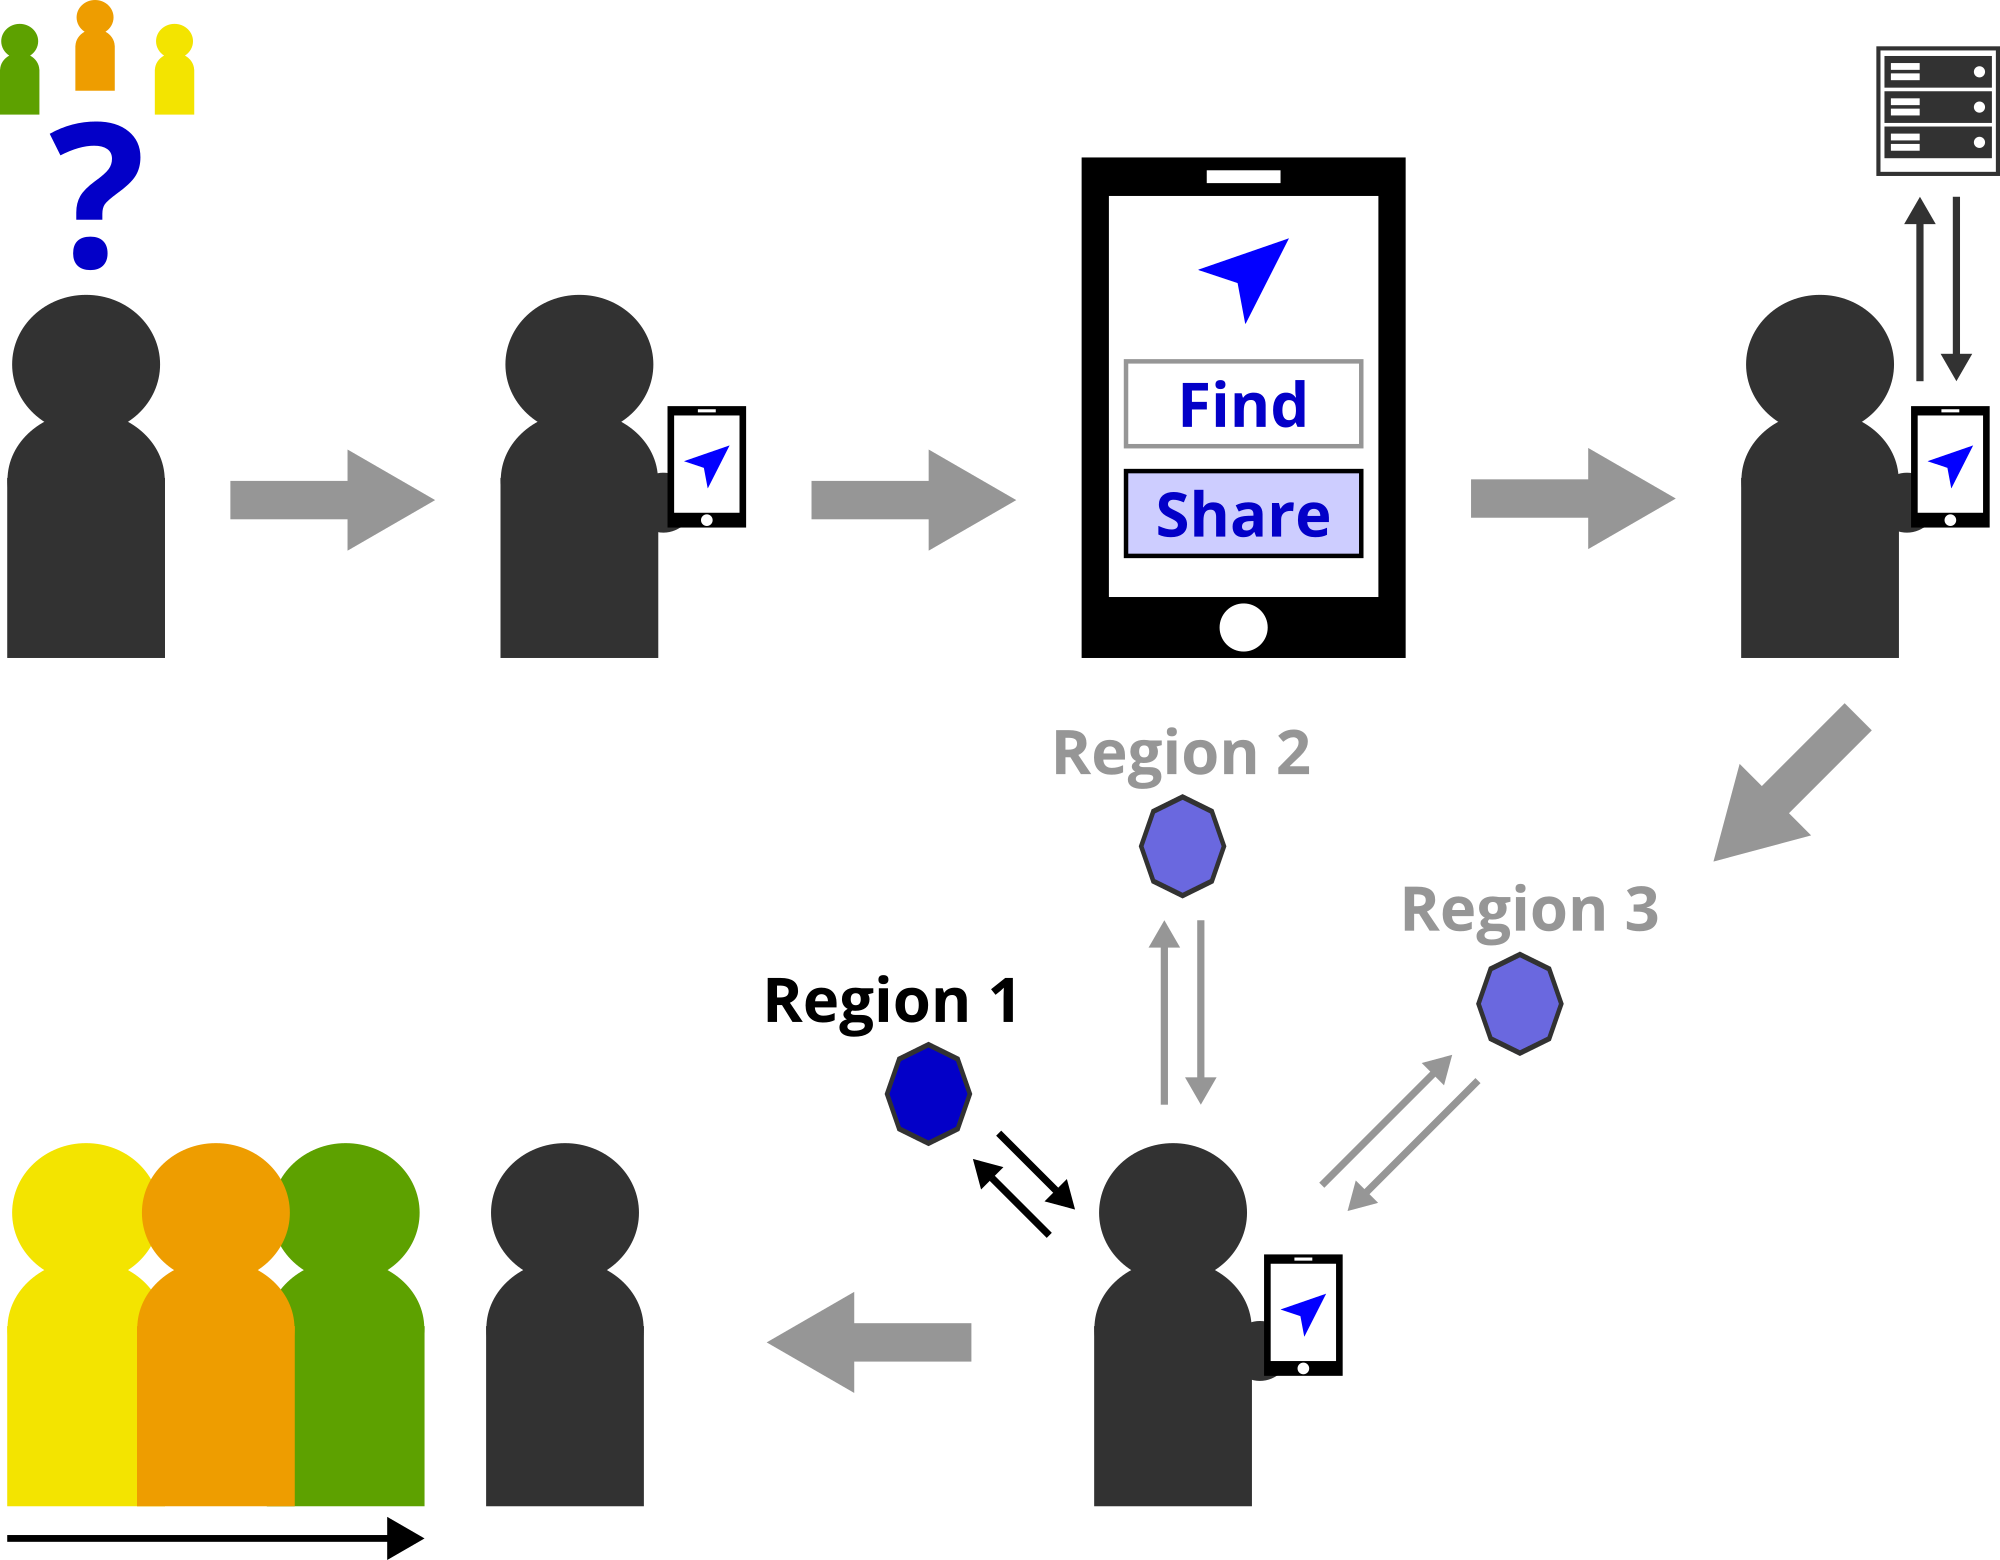
\includegraphics[width=.6\textwidth]{user-story}
	
	\end{center}
    
    \textbf{Main goal:} indoor region-based navigation

\end{frame}

\section{Our approach}

\begin{frame}{Our approach - vision}

    \begin{center}
        \only<1>{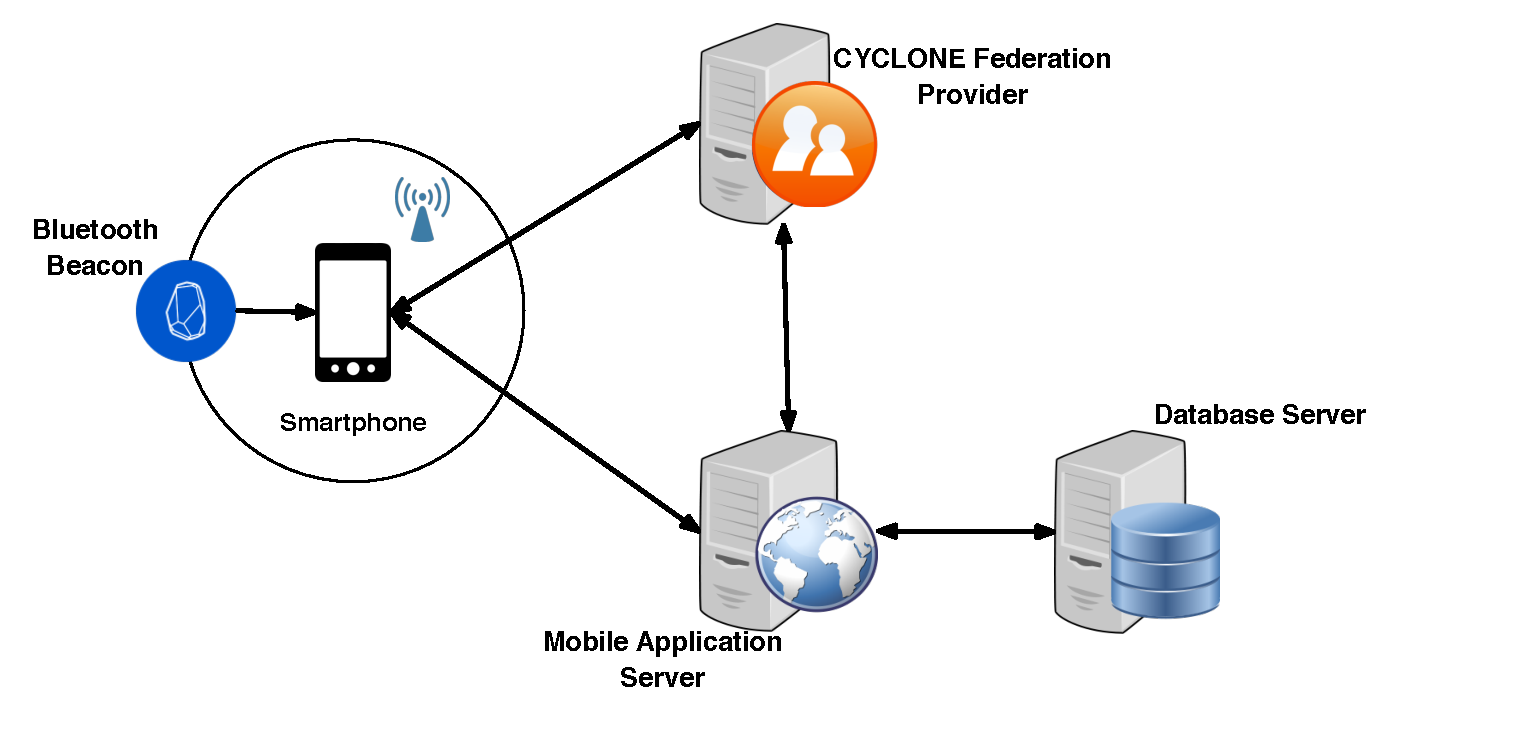
\includegraphics[width=\textwidth]{architecture}}%
        \only<2>{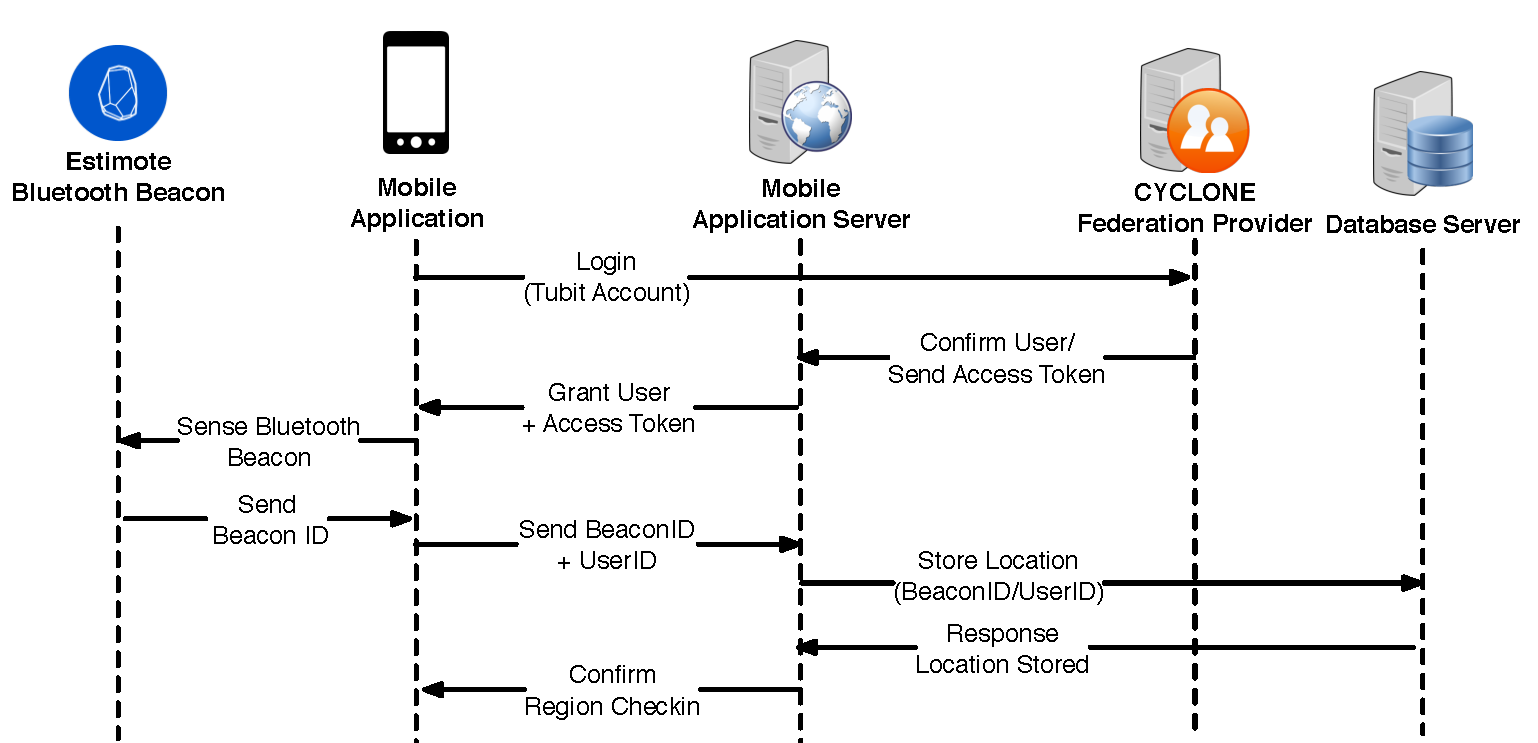
\includegraphics[width=\textwidth]{sequencediagram_sharelocation_extended_updated_arrow}}
    \end{center}

\end{frame}

\section{Timeline}

\begin{frame}{Possible future work}

	\begin{itemize}
        \item Smart watch application
        \item Live Indoor-Location Feedback Navigation
        \item D2D Indoor-Navigation via Virtual Beacons
    \end{itemize}

\end{frame}

\begin{frame}{Timeline}

    \begin{center}
    
    	\begin{tabular}{ l | l }
    	
    		\textbf{week}	&	\textbf{topic} \\
            \midrule
            21.10			&	research \\
            04.11			&	technology overview \\
            18.11			&	prototype of iOS and Android app \\
            02.12			&	1st iteration (basic pinning - min. functions) \\
            16.12			&	2nd iteration \\
            30.12			&	3rd iteration (basic positioning - min. func.) \\
            13.01			&	4th iteration \\
            27.01			&	preperation for final presentation \\
            10.02			&	final presentation \\
        \end{tabular}

    \end{center}

	\begin{itemize}
		\item 2 week sprints
	\end{itemize}

\end{frame}

\begin{frame}{Questions?}

	\begin{center}
	
		{\Huge Do you have questions?}
        
    \end{center}

\end{frame}

\begin{frame}[allowframebreaks]{References}

	\nocite{*}
	{\tiny \bibliography{references}}

\end{frame}

\end{document}